\documentclass[a4paper, 11pt, twoside]{book}
\usepackage[a4paper]{geometry}
\usepackage{textcomp}
\usepackage{color}
\usepackage{url}
\usepackage{amsfonts}
\usepackage{float}
\usepackage{booktabs}
\usepackage{longtable}
\usepackage{makeidx}
\usepackage{fancyhdr}
\usepackage[times]{quotchap}
\usepackage{amsmath}
\usepackage{listings}
\usepackage{fancybox}
\usepackage{enumitem}
\usepackage[toc,page]{appendix} % appendice
\usepackage{dirtree}  % struttura directory
\usepackage{hyphenat}

%%%%%%  BIBLIOGRAFIA  %%%%%%
\usepackage[
backend=biber,
style=numeric
]{biblatex}
\addbibresource{content/biblio.bib}

%%%%%%  APPENDICE  %%%%%%
\renewcommand{\appendixname}{Appendice}
\renewcommand{\appendixtocname}{Appendice}
\renewcommand{\appendixpagename}{Appendice}

%% Aggiunge una linea al di sotto di ogni sezione principale
\usepackage[calcwidth]{titlesec}
\titleformat{\section}[hang]{\sffamily\bfseries}
 {\Large\thesection}{12pt}{\Large}[{\titlerule[0.4pt]}]

%% Gestisce la grafica a seconda che si usi latex o pdflatex
\newif\ifpdf
\ifx\pdfoutput\undefined
\pdffalse % no pdflatex
\else
\pdfoutput=1 % pdflatex
\pdftrue
\fi
%
\ifpdf
\usepackage[pdftex]{floatflt,graphicx}
\DeclareGraphicsExtensions{.pdf,.mps,.png,.jpg}
\graphicspath{{img/}}
\usepackage[hidelinks,pdftex]{hyperref}
\else
\usepackage{floatflt,graphicx}
\DeclareGraphicsExtensions{.eps}
\fi
\usepackage{subfig}
\usepackage{adjustbox}
\usepackage{multirow}
\usepackage[utf8]{inputenc} % per accenti

%%%%%%%%%%%%% NUOVI COMANDI E IMPOSTAZIONI %%%%%%%%%%%
\newenvironment{mcquote}
  {\begin{list}{}{
      \setlength{\rightmargin}{\leftmargin}}
         \item[]``\ignorespaces}
  {\unskip''\end{list}}
  
\newcommand{\mcchap}[2]{\protect{
 \chapter{#1}
 \label{#2}
}}

%% Gestione header: no header sulle dispari bianche
\makeatletter
\def\cleardoublepage{\clearpage\if@twoside \ifodd\c@page\else%
    \hbox{}%
    \thispagestyle{empty}%              % Empty header styles
    \newpage%               commentare per togliere pagine bianche
    \if@twocolumn\hbox{}\newpage\fi\fi\fi}
\makeatother


\newcommand{\placetextbox}[3]{% \placetextbox{<horizontal pos>}{<vertical pos>}{<stuff>}
  \setbox0=\hbox{#3}% Put <stuff> in a box
  \AddToShipoutPictureFG*{% Add <stuff> to current page foreground
    \put(\LenToUnit{#1\paperwidth},\LenToUnit{#2\paperheight}){\vtop{{\null}\makebox[0pt][c]{#3}}}%
  }%
}%


%%%%%%%%%%%%%%%% METADATI DOCUMENTO %%%%%%%%%%%%%%%%%%
\date{}

%%%%%%%%%%%%%%%%%% INIZIO DOCUMENTO %%%%%%%%%%%%%%%%%%
\begin{document}
\pagestyle{empty}

%% Pagina del titolo
  \begin{titlepage}
  \begin{center}
  \begin{large}
  {\fontsize{20}{18}\selectfont\vspace*{0.50cm}Università dell'Insubria}\\
  \vspace{.1cm}
  Dipartimento di Scienze Teoriche e Applicate - DiSTA\\
  \vspace{.1cm}
  Corso di Laurea Triennale in Informatica
  \end{large}
  
  \vspace{1cm}
  \begin{figure}[h]
    \begin{center}
      
\includegraphics[scale=0.16]{insubria}
    \end{center}
  \end{figure}

    {\fontsize{25}{25}\usefont{OT1}{phv}{bc}{n}\selectfont\par
    Realizzazione di una Dashboard di Business Intelligence per la pandemia da COVID-19}
    \par    
    \vspace{2.4cm}
    \begin{large}
    Tesi di:\\
    Alessandro Riva\\
    Matricola 734572\\
    \vspace{2.3cm}
    Relatore:\\
    Prof. Davide Tosi\\
    \vfill
    Marzo, 2021
    \end{large}
    

  \end{center}
\end{titlepage}
  \cleardoublepage{}
  ~\\
~\\
~\\
~\\
~\\
~\\
~\\
~\\
~\\
~\\
~\\
~\\
~\\
~\\
~\\
~\\
~\\
~\\
~\\
~\\
~\\
~\\
~\\
~\\
~\\
~\\
~\\
~\\
~\\
~\\
~\\
~\\
~\\
\begin{flushright}
\emph{Per questo traguardo devo ringraziare innanzitutto i miei genitori, che mi hanno sostenuto e incoraggiato durante questi anni. Senza mia madre e mio padre, non avrei avuto la possibilità di studiare e di scrivere questo elaborato.}
\end{flushright}
  
%% Indice ed elenchi  
  \pagenumbering{roman}
  \setcounter{page}{1}
  \setcounter{tocdepth}{3}
  \renewcommand*\contentsname{Contenuti}
  \tableofcontents
  
%% Inizio capitoli
  \mainmatter{}

%% Capitoli
  \pagestyle{fancy}
  \Large % aumenta la dimensione del carattere
  \setlength{\parskip}{1em} % spazio paragrafi
  \setlength{\parindent}{0pt} % indentazione dei paragrafi
  \renewcommand{\baselinestretch}{1.2} % spaziatura tra le righe
  \renewcommand{\chaptermark}[1]{\markboth{#1}{}} 
  \renewcommand{\sectionmark}[1]{\markright{\thesection\ #1}} 
  \fancyhf{} % delete current setting for header and footer 
  \fancyhead[LE,RO]{\bfseries\thepage} 
  \fancyhead[LO]{\bfseries\rightmark} 
  \fancyhead[RE]{\bfseries\leftmark} 
  \renewcommand{\headrulewidth}{0.8pt} 
  \renewcommand{\footrulewidth}{0pt} 
  \renewcommand{\figurename}{Fig.} % cambio nome figura
  %\renewcommand{\headheight}{13.59999pt}
  \addtolength{\headheight}{0.5pt} % make space for the rule 
  \fancypagestyle{plain}{% 
  \fancyhead{} % get rid of headers on plain pages
  \fancyfoot[C]{\bfseries \thepage}
  \renewcommand{\headrulewidth}{0pt} % and the line 
  } 

\cleardoublepage{}
\setcounter{page}{1}
\mcchap{Introduzione}{cap:intro}

Viviamo in un mondo sempre più data-driven. La quantità di dati prodotti ogni giorno cresce in modo esponenziale, quindi è importante gestire questa mole di dati nel modo più efficiente ed efficace possibile, sfruttando le nuove tecnologie.
I dati sono fondamentali per prendere decisioni in modo rapido.

\section{Scopo del lavoro}

Giornalmente il dipartimento di Protezione Civile comunica i numeri dei contagi relativi alla pandemia di Covid 19.
Per una migliore consultazione si è pensato di sviluppare  un’applicazione in grado di rappresentare i dati in modalità grafica, per facilitare la lettura e la comprensione dell’andamento della pandemia.
Lo scopo del seguente elaborato è quello di illustrare la struttura dell'applicazione creata per la realizzazione di questo servizio accessibile online attraverso l’elaborazione dei dati relativi all’emergenza di Coronavirus Covid-19 utilizzando dei grafici interattivi.

\section{La Business Intelligence}
\subsection{Definizione}
La Business Intelligence o BI consiste nella trasformazione dei dati grezzi in informazioni utili e significative.
La Business Intelligence si può definire anche come un insieme di metodologie che spaziano da tutti i processi necessari per la raccolta dei dati, alle architetture e alle tecnologie  utilizzate per implementare tali processi, che trasformano dati in informazioni utili.

\subsection{L'importanza dei dati}
Nelle prime settimane della pandemia, la conoscenza della malattia e del suo trattamento è stata generata dalla condivisione di osservazioni aneddotiche e piccole serie di casi.

\noindent Nonostante gli operatori sanitari utilizzano la tecnologia moderna per comunicare, mai prima d'ora l'incapacità di costruire sistemi solidi di condivisione dei dati per analisi quasi in tempo reale su larga scala nell'assistenza sanitaria è stata più ovvia.

\noindent Nell'era delle cartelle cliniche elettroniche, i dati fisiologici, di laboratorio, di imaging, del processo decisionale e del trattamento vengono aggiornati continuamente. Le inferenze tratte da questi dati possono supportare le indagini epidemiologiche e guidare i protocolli di trattamento quando i dati degli studi clinici non sono disponibili o insufficienti per la gestione di una situazione in così rapida evoluzione.

\noindent Con il diffondersi della pandemia, i dati si accumulano, ma tendono a restare isolati all'interno dei sistemi ospedalieri. Per la lotta contro COVID-19 potrebbe essere molto utile condividere i dati disponibili con istituti di ricerca ed aziende farmaceutiche.

\noindent Sfortunatamente, i dati COVID-19 a livello di paziente non sono disponibili pubblicamente. 
Non esiste un database di questo tipo tecnologia o precedenti. 

\noindent Nonostante la tecnologia, non esiste un database globale liberamente accessibile, pertanto i dato sul Covid-19 a livello di paziente non sono disponibili pubblicamente.





\mcchap{Contesto del lavoro}{cap:contesto}

\noindent Il 30 dicembre 2019, Li Wenliang, un oftalmologista dell’ospedale di Wuhan, ha condiviso online in una chat dei suoi amici la notizia di un nuovo virus sospetto simile alla SARS.
Il 3 gennaio 2020, Li fu intimato dalla polizia di non di diffondere false notizie online.

\noindent Li fu infettato dal nuovo virus e morì poco dopo, il 7 febbraio all’età di 33 anni.
Il virus scoperto in Cina, si diffuse rapidamente, fino a diventare un'emergenza sanitaria a livello globale.
A causa dell’elevata contagiosità del virus, e la necessità di cure in terapia intensiva, gli ospedali divennero presto sotto pressione a causa del numero elevato di ricoveri.
L'epidemia divenne presto una pandemia nonostante i vari governi del mondo misero in atto diverse misure restrittive per contenere il propagarsi del virus.

\noindent I vari governi del mondo nonostante misero in atto diverse misure per cercare di contenere il propagarsi del virus, l'epidemia divenne in una pandemia globale.

\noindent Il seguente lavoro di tesi, in collaborazione con il Professor Davide Tosi Ricercatore dell’Università degli Studi dell’Insubria di Varese, ha lo scopo di illustrare mediante dei grafici interattivi l’evoluzione in tempo reale dei dati dell’epidemia in Italia, e rappresenta il prosieguo del lavoro di tesi intrapreso dalla Dottoressa Alice Schiavone sul calcolo degli indici di contagio R0(t). % inserire citazione!
\mcchap{Obiettivi}{cap:obiettivi}

L’obiettivo di questo progetto è la realizzazione di una dashboard in grado di mostrare le informazioni sulla pandemia di Coronavirus Covid-19 in maniera ottimale e immediata.

Il termine \emph{dashboard} comprende un insieme di oggetti grafici che, strutturati e raffigurati in un determinato modo, rendono visibile in tempo reale molte informazioni anche di diversa natura e complessità. 
La dashboard deve avere le seguenti caratteristiche:

\begin{itemize}
    \item Rappresentare in modo semplice e chiaro i dati sulla pandemia;
    \item Aggiornarsi automaticamente con la pubblicazione dei nuovi dati;
    \item Grafici interattivi
\end{itemize}
\mcchap{La visualizzazione dati}{cap:breveStoria}

\section{Cos'è la visualizzazione dati }
La rappresentazione grafica dei dati o in inglese \emph{data visualization} è l’attività di comunicazione realizzata tramite la proiezione di dati in una forma grafica strutturata.

\section{Breve storia}

Con la tecnologia moderna, la visualizzazione di dati non è mai stata così semplice.
Con pochi click si può trasformare un enorme tabella di dati grezzi in un diagramma accattivante e semplice da interpretare.
Rappresentare i dati sotto forma di grafici, fornisce una via molto rapida per rendere comprensibile e far capire il proprio punto di vista.
Molte tecniche di visualizzazione dati che si usano oggi sono state inventate durante la prima rivoluzione industriale.
Quello che può sembrare semplice e ovvio al giorno d’oggi, come un grafico a linea o a barre, sarebbe stato strano e incomprensibile 200 anni fa.


\noindent Nel 18esimo secolo uno tra i primi pionieri della visualizzazione dati fu William Playfair, uno statista scozzese, visse nel periodo dell’Illuminismo e che introdusse la rappresentazione grafica in statistica ed economia.

\noindent In pochi anni introdusse modi innovativi di rappresentare graficamente i dati, oggi passati alla storia. Nella sua opera del 1786 dal titolo “The Commercial and Political Atlas” incluse 44 grafici, tutti particolarmente “creativi” per l’epoca, come dimostra quello che illustra la differenza tra import ed export dell’economia inglese.

\noindent Ai tempi di Playfair, i dati venivano presentati in tabelle asettiche di non facile lettura con poca attenzione per la loro interpretazione. Per comprenderli, non c’erano scorciatoie intuitive, dove solo dopo un laborioso lavoro di esaminare attentamente i numeri, ricordare, copiare e confrontare i dati.

\noindent Poi, nel 1765, arrivò il diagramma temporale di Joseph Priestley, che mostrava le vite sovrapposte di vari statisti e filosofi classici. Invece di elencare semplicemente nomi, anni di nascita e anni di morte, Priestley li tracciò su una linea temporale, rendendo immediatamente visibile quali personaggi storici fossero contemporanei.

\begin{figure}[htp]
    \centering
    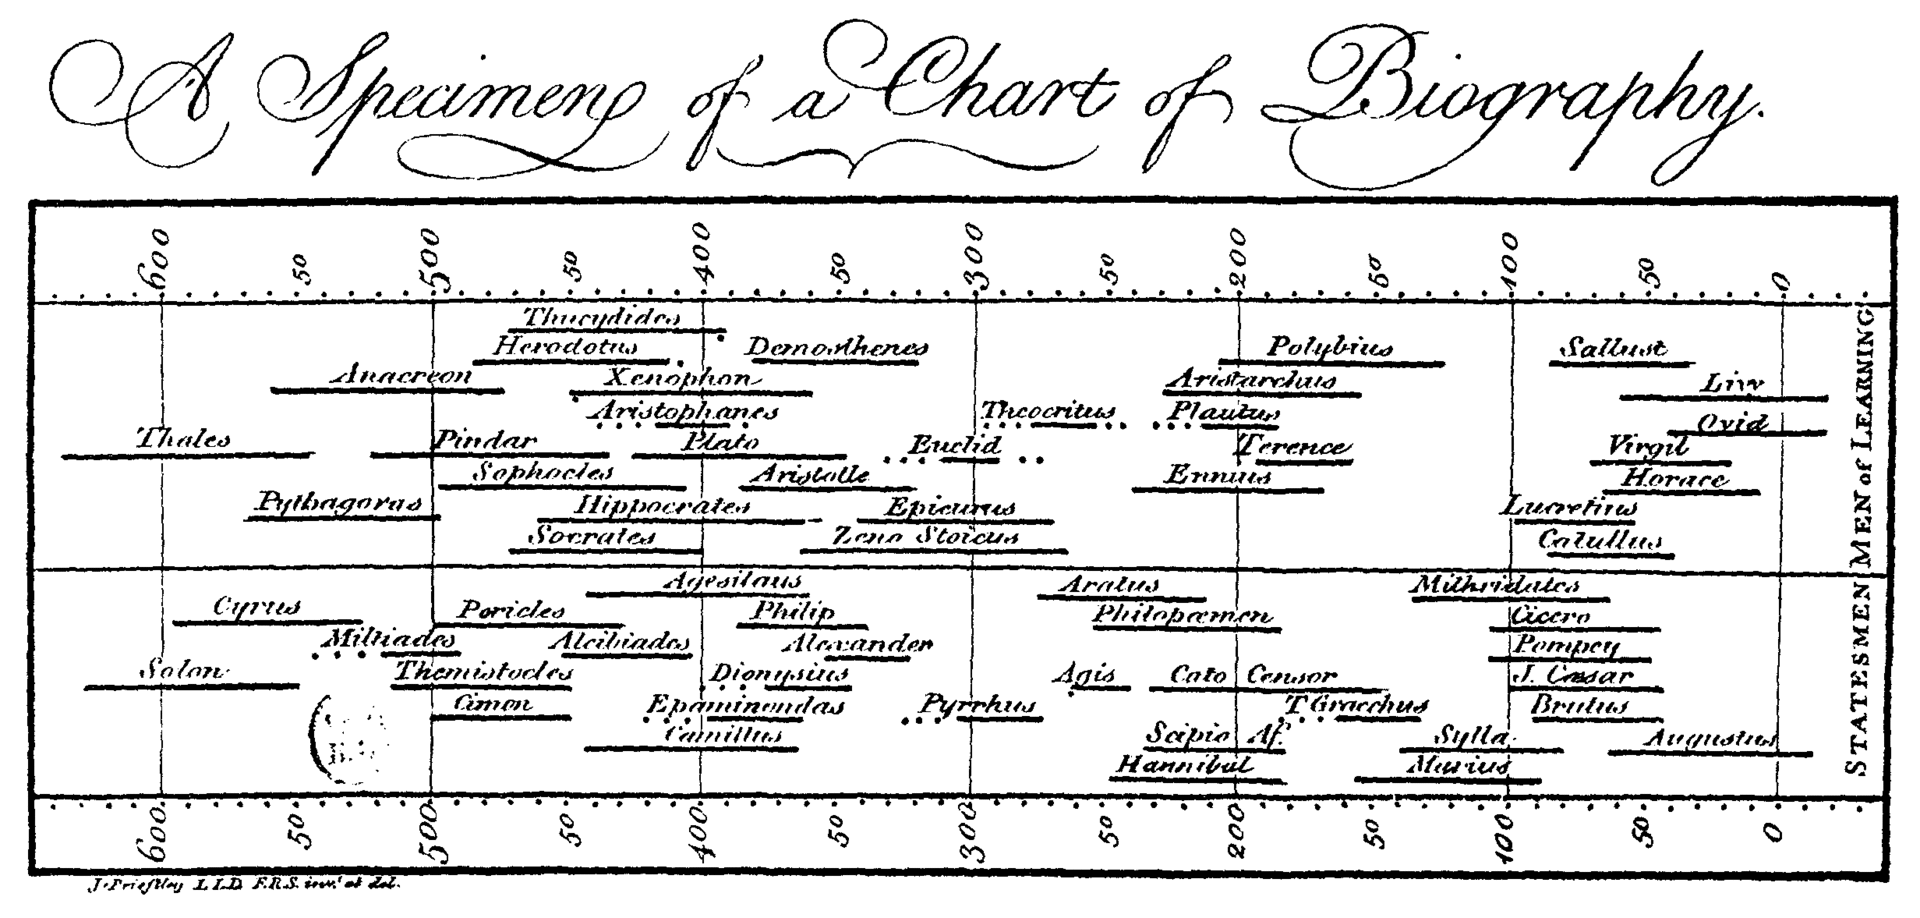
\includegraphics[width=10cm]{PriestleyChart}
    \caption{Joseph Priestley — Grafico sequenza temporale}
    \label{fig:PriestleyChart}
\end{figure}

\noindent Queste sequenze temporali si sono rivelate un successo e hanno ispirato direttamente l'invenzione del grafico a barre di Playfair, che apparve per la prima volta nel suo Atlante commerciale e politico.

\begin{figure}[htp]
    \centering
    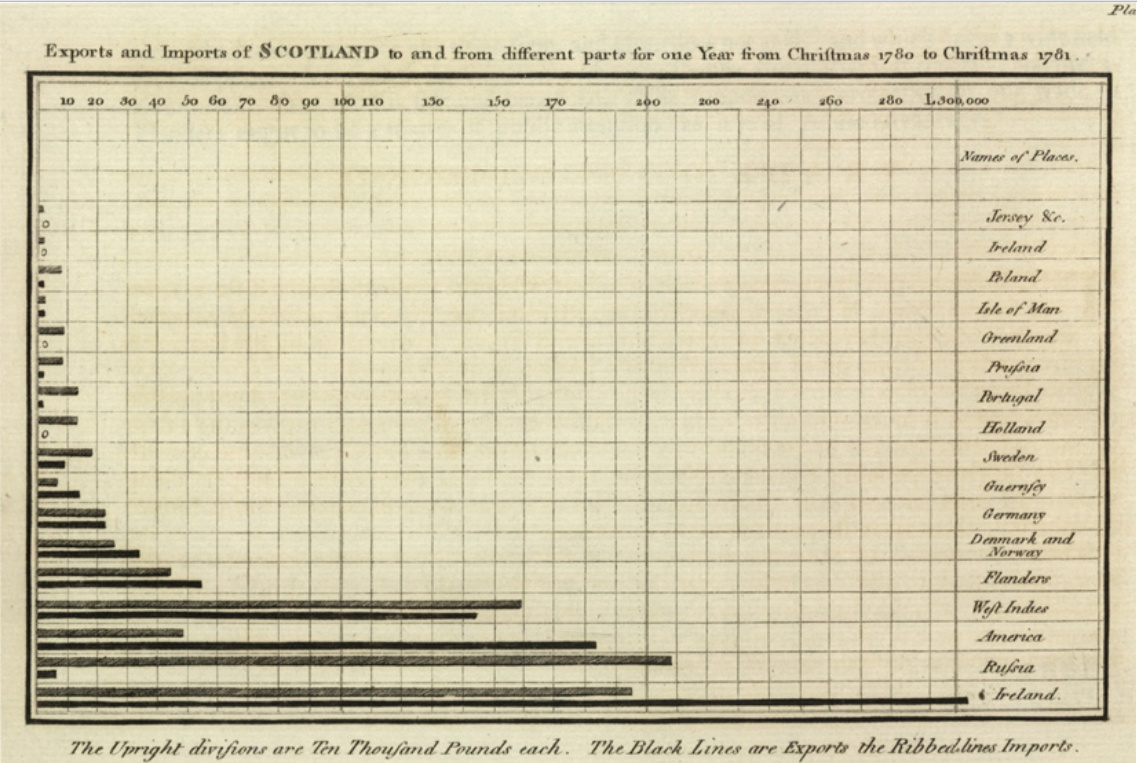
\includegraphics[width=9cm]{Playfair_chart}
    \caption{William Playfair — Atlante Politico e Commerciale}
    \label{fig:playfair_chart}
\end{figure}

\noindent Quindici anni dopo, Playfair era tornato con con il grafico a torta a volte controverso e varie combinazioni creative. È sorprendente pensare che, più di duecento anni dopo, le idee di un uomo costituiscano ancora la maggior parte delle opzioni grafiche in un software di visualizzazione dei dati all'avanguardia.

\begin{figure}[htp]
    \centering
    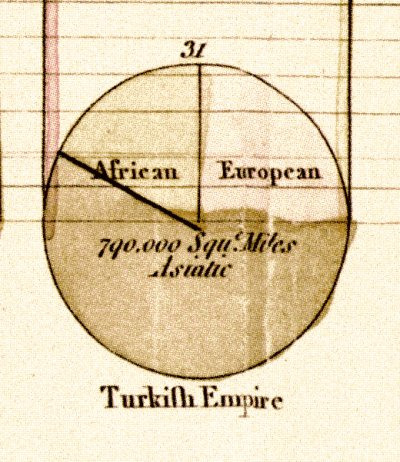
\includegraphics[width=6cm]{playfair_piechart}
    \caption{William Playfair — Grafico a torta}
    \label{fig:playfair_piechart}
\end{figure}





\mcchap{Design e sviluppo della soluzione}{cap:designSviluppo}

\section{Origine dei dati}
La principale fonte di dati riguardanti la diffusione della pandemia da COVID-19 in Italia è il Dipartimento della Protezione Civile, che giornalmente a partire dal 24 febbraio pubblica i relativi dati sul repository Github\cite{repository}.

Alcuni dati disponibili sul repository sono i seguenti:
\begin{itemize}
    \item Ricoverati con sintomi: numero di soggetti ricoverati non in terapia intensiva.
    \item Terapia intensiva: Numero di soggetti ricoverati in terapia intensiva.
    \item Totale ospedalizzati: Totale dei soggetti ricoverati in ospedale.
    \item Isolamento domiciliare: Soggetti ricoverati presso la propria abitazione.
    \item Deceduti: Persone decedute positive al virus.
    \item Tamponi: numero di tamponi effettuati (antigenici + molecolari)
\end{itemize}


\begin{figure}[htp]
    \centering
    
\includegraphics[width=5cm]{logo_dpc}
    \caption{Logo del Dipartimento della Protezione Civile}
\end{figure}


\section{Tecnologie utilizzate}
In questa sezione verranno elencate alcune delle tecnologie utilizzate per lo sviluppo del progetto.

\subsection{Python}
Python è un linguaggio di programmazione dinamico orientato agli oggetti utilizzabile per molti tipi di sviluppo software, è completamente gratuito ed è utilizzabile senza restrizioni di copyright.\\
Python è un linguaggio portabile sviluppato in ANSI C, è caratterizzato da una sintassi essenziale, ma consente lo sviluppo di applicazioni molto complesse.\\
È multipiattaforma e quindi utilizzabile su diversi  sistemi operativi quali Windows, MacOS e GNU/Linux.
Offre un forte supporto all'integrazione con altri linguaggi e programmi, dispone di una estesa libreria standard e funzioni matematiche integrate, che semplificano il calcolo dei problemi matematici e l'esecuzione dell'analisi dei dati.

\begin{figure}[htp]
    \centering
    
\includegraphics[width=4cm]{python_logo}
    \caption{Logo di Python}
\end{figure}
\noindent Per lo sviluppo del progetto è stato utilizzato interamente il linguaggio Python versione 3.8.

\subsection{Plotly}

Plotly è una libreria Python open source  per la creazione di grafici interattivi, supporta oltre 40 tipologie diverse di grafici che consentono l’applicazione in vari campi scientifici, tra i quali la statistica, la finanza, e la geografia.
Plotly basa il suo funzionamento sulla libreria Javascript plotly.js, che permette agli utenti Python di realizzare stupende applicazioni di visualizzazione dati interattive, che si possono mostrare in un file HTML indipendente, in un Notebook Jupyter\footnotemark, oppure all’interno di una applicazione web utilizzando Dash.
\footnotetext{Jupyter Notebook è un'applicazione web open source che consente di creare e condividere documenti che contengono codice Python eseguibile in tempo reale, equazioni, visualizzazioni.}

\begin{figure}[htp]
    \centering
    
\includegraphics[width=4cm]{plotly_logo}
    \caption{Logo di Plotly}
\end{figure}

\subsection{Pandas}
Pandas è una libreria Python open source, adatta per l’analisi e la manipolazione di dati in formato sequenziale o tabellare.
Pandas consente il Caricamento e il salvataggio di formati standard per dati tabellari, come CSV (Comma-separated Values).
Una delle strutture dati utilizzate da Pandas prende il nome di DataFrame, una struttura dati bi-dimensionale, con dimensione variabile che può contenere dati eterogenei.
\begin{figure}[htp]
    \centering
    
\includegraphics[width=4cm]{pandas_logo}
    \caption{Logo di Pandas}
\end{figure}

\subsection{Dash}
Dash è un framework Python ideato per la costruzione di applicazioni web di analytics, si appoggia a Flask\footnotemark, Plotly.js e react.js\footnotemark.
Dash è ideale per la costruzione di applicazioni di visualizzazione dati molto personalizzabili, usando soltanto il linguaggio Python. 
È particolarmente indicato per chiunque lavori con i dati in Python.
Attraverso l’utilizzo di semplici pattern, Dash semplifica notevolmente la costruzione di applicazioni basate su web, come nel caso della dashboard, in quanto non è necessario conoscere approfonditamente le tecnologie e i protocolli che ne determinano il funzionamento.
\footnotetext{Flask è un framework leggero sviluppato da Armin Ronacher per applicazioni web WSGI
(Web Server Gateway Interface).}
\footnotetext{React è una libreria JavaScript per la creazione di interfacce utente.}


\begin{figure}[htp]
    \centering
    
\includegraphics[width=4cm]{dash_logo}
    \caption{Logo di Dash}
\end{figure}


\subsection{Github}
\noindent GitHub è un servizio web basato su cloud che aiuta gli sviluppatori ad archiviare e gestire il loro codice e a tracciare e controllare le modifiche.

\noindent Git è un sistema che consente il controllo delle versioni e permette a più sviluppatori di collaborare allo stesso progetto contemporaneamente.
\noindent In sostanza Github, semplifica l’utilizzo del software a riga di comando Git per il controllo delle versioni e la collaborazione.


\begin{figure}[htp]
    \centering
    
\includegraphics[width=3cm]{github_logo}
    \caption{Logo di Github}
\end{figure}

\subsection{Docker}
\noindent Docker è un progetto open source nato con lo scopo di automatizzare la distribuzione di applicazioni sotto forma di “contenitori” detti container.
I container hanno al loro interno tutto il necessario per la corretta esecuzione dell’applicazione, incluse librerie, strumenti di sistema, codice e runtime.

\begin{figure}[htp]
    \centering
    
\includegraphics[width=4cm]{docker_logo}
    \caption{Logo di Docker}
\end{figure}

\noindent Un container è basato su un’immagine che rappresenta tutto il suo contenuto e definisce quale applicativo sarà eseguito al suo interno. 
Per il progetto è stato scelto Docker in quanto consente di isolare una dashboard dalle altre e pertanto semplifica il processo di distribuzione e aggiornamento.

\section{Lo sviluppo}
Lo sviluppo del progetto è iniziato partendo dai dati contenuti in un foglio di calcolo Excel fornito dal professore, dal quale sono state estrapolate le formule necessarie per l’elaborazione degli stessi atti alla costruzione della dashboard.

\subsection{Calcoli dei dati}
I calcoli vengono effettuati direttamente nella struttura DataFrame di Pandas
\begin{figure}[htp]
    \centering
    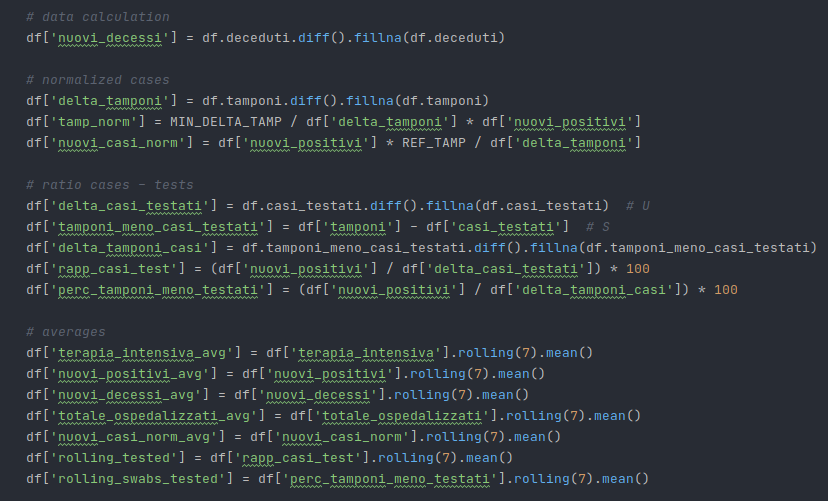
\includegraphics[width=10cm]{data_calculation}
    \caption{Codice Python per il calcolo dei dati}
\end{figure}


\subsection{Diagramma di attività}
Un diagramma di attività UML è un diagramma di flusso che rappresenta il flusso del programma da un'attività all'altra,
da un punto iniziale (punto nero pieno) a un punto finale.

\begin{figure}[htp]
    \centering
    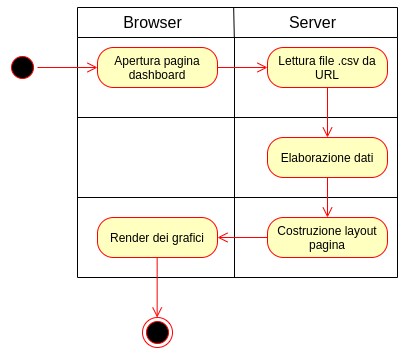
\includegraphics[width=7cm]{activity}
\end{figure}

\subsection{Organizzazione file}
Una applicazione Dash è composta essenzialmente da un singolo programma Python.
Viene utilizzata una versione minimale del framework Bootstrap\footnotemark, questo assicura dei tempi di caricamento della pagina decisamente più rapidi.
\footnotetext{Bootstrap è un framework CSS utilizzato per la semplificare la gestione dello stile della dashboard}

\begin{figure}
\centering
\begin{minipage}{.3\linewidth}
\dirtree{%
.1 italy.
.2 assets.
.3 bootstrap.min.css.
.2 dash\_italy.py.
}
\caption{Struttura file dashboard Italia}
\end{minipage}\hfill
\begin{minipage}{.65\linewidth}
\dirtree{%
.1 lombardia.
.2 assets.
.3 bootstrap.min.css.
.2 dash\_lombardia.py.
}
\caption{Struttura file dashboard Italia}
\end{minipage}
\end{figure}

% seconda figura

\begin{figure}
\centering
\begin{minipage}{.3\linewidth}
\dirtree{%
.1 regioni.
.2 assets.
.3 bootstrap.min.css.
.3 img.
.4 Abruzzo.png.
.4 Basilicata.png.
.4 Calabria.png.
.4 ....
.2 dash\_regioni.py.
}
\caption{Struttura file dashboard regioni}
\end{minipage}\hfill
\end{figure}

\section{Grafico di esempio}
Come scritto precedentemente, i grafici sono interattivi.
Sul grafico è possibile agire sull'intervallo di tempo selezionato (punto 1), oppure mostrare e nascondere le varie parti cliccando sulla legenda (punto 2).
\begin{figure}[htp]
    \centering
    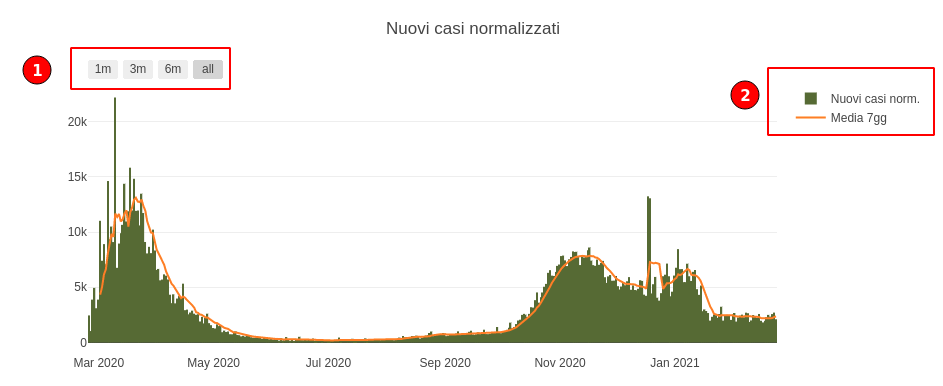
\includegraphics[width=14cm]{chart_explained}
    \caption{Esempio grafico}
\end{figure}

\section{Problemi riscontrati}
I dati forniti dal Dipartimento della Protezione Civile non sono esenti da errori, ciò può essere dovuto a errori di trascrizione oppure a causa di comunicazioni parziali o in ritardo dal parte delle regioni.

\noindent Alcune serie di dati, come ad esempio quelli cumulativi come guariti, deceduti, totale casi e tamponi, che dovrebbero essere strettamente crescenti, alcune volte non lo sono.

\subsection{Errore nei tamponi}
Il 17 dicembre 2020 è stato registrato un valore incorretto nel valore cumulativo dei tamponi, ciò ha causato un anomalia nel grafico dei casi normalizzati.\\
Per la correzione di questo problema è stato effettuato un intervento di pulizia del dato.
Il dato "incriminato" è stato sostituito con la media tra il giorno precedente e quella del giorno successivo.
\begin{figure}[htp]
    \centering
    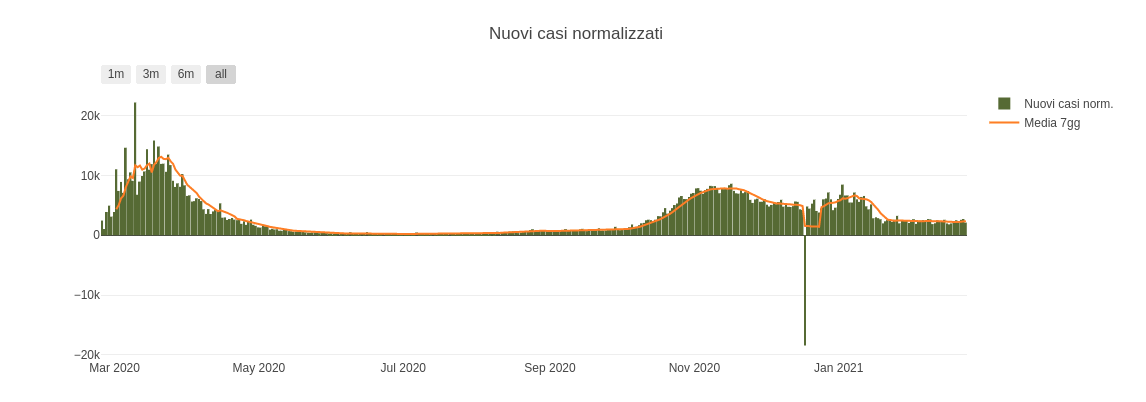
\includegraphics[width=14cm]{chart_problem}
    \caption{Problema causato dal valore incorretto dei tamponi}
\end{figure}



\mcchap{Le dashboard}{cap:dashboard}
In questo capitolo, a titolo di esempio verranno presentate delle immagini relative alle schermate estratte dall'applicazione.
È possibile visualizzare l’andamento dei contagi riferito a 1, 3, 6 mesi e per tutto il periodo di riferimento a partire da marzo 2020.
Tutti i grafici contenuti nella dashboard, sono interattivi.
Passando con il cursore del mouse sopra al grafico, vengono evidenziate le barre che indicano il numero dei contagi per quel determinato giorno.
Sul grafico è possibile agire sull'intervallo di tempo selezionando uno dei pulsanti indicati nel riquadro 1 della figura, oppure cliccando sulla legenda del riquadro 2, cambiare la configurazione delle tracce.
\begin{figure}[htp]
    \centering
    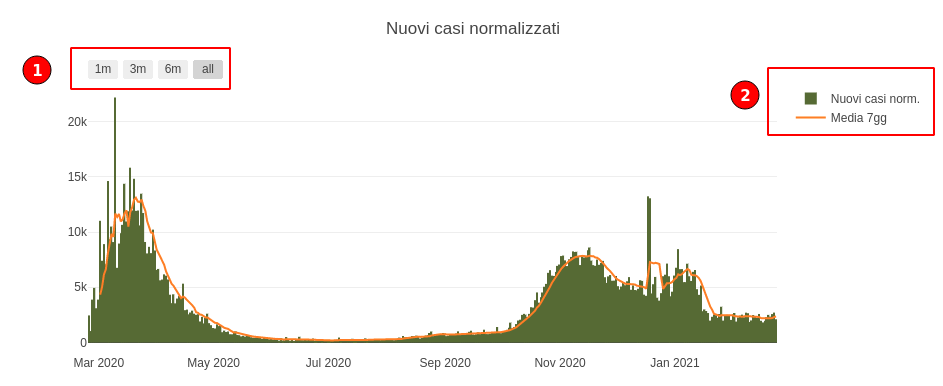
\includegraphics[width=14cm]{chart_explained}
    \caption{Esempio grafico}
\end{figure}
\section{Dashboard Italia}
Nella dashboard Italia sono presenti nove diversi grafici che illustrano l’andamento della pandemia attraverso le curve di contagi, le ospedalizzazioni, le terapie intensive e i decessi.
\subsection{Nuovi casi}
La figura \ref{fig:nuovi_casi} mostra il numero di nuovi casi giornalieri in Italia a partire dall'inizio della pandemia.
In ascissa sono riportati i giorni, e in ordinata il numero dei nuovi casi riportati in quel determinato giorno.
\begin{figure}[htp]
    \centering
    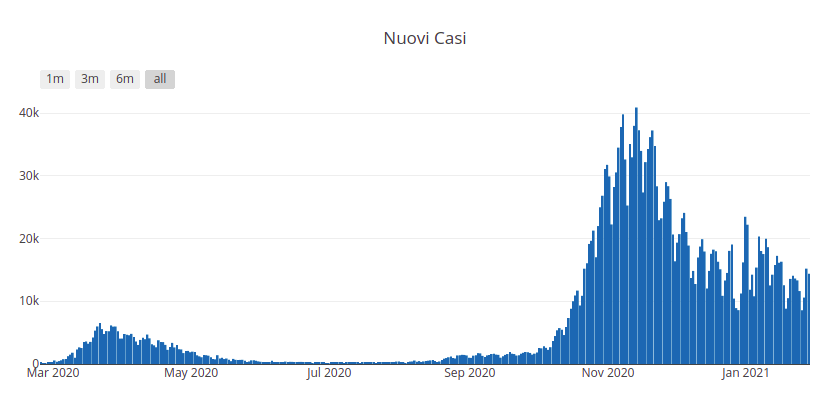
\includegraphics[width=14cm]{nuovi_casi}
    \caption{Nuovi casi}
    \label{fig:nuovi_casi}
\end{figure}

\subsection{Totale casi}
Nella figura \ref{fig:totale_casi} sono rappresentati i casi totali delle persone che hanno contratto il virus, che comprende gli attuali positivi, i guariti e i decessi.
\begin{figure}[htp]
    \centering
    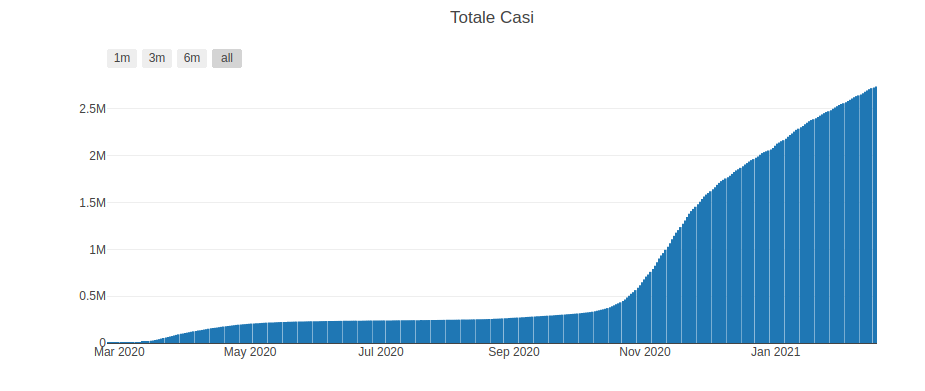
\includegraphics[width=14cm]{totale_casi}
    \caption{Totale casi}
    \label{fig:totale_casi}
\end{figure}

\subsection{Isolamento domiciliare}
Nella figura \ref{fig:isolamento_domiciliare} è raffigurato il grafico delle persone che si trovano in isolamento presso il loro domicilio.
\begin{figure}[htp]
    \centering
    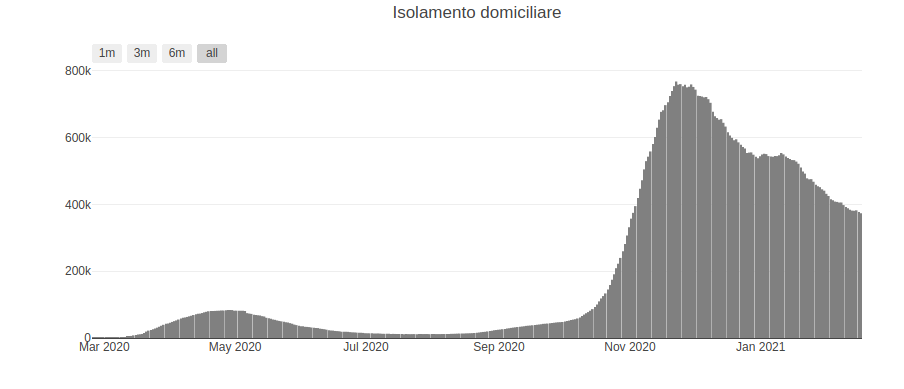
\includegraphics[width=14cm]{isolamento_domiciliare}
    \caption{Isolamento domiciliare}
    \label{fig:isolamento_domiciliare}
\end{figure}

\subsection{Terapia intensiva}
La figura \ref{fig:terapia_intensiva} mostra l'andamento dei pazienti ricoverati in ospedale in terapia intensiva dall'inizio della pandemia.
La linea indica la media mobile a 7 giorni.
\begin{figure}[htp]
    \centering
    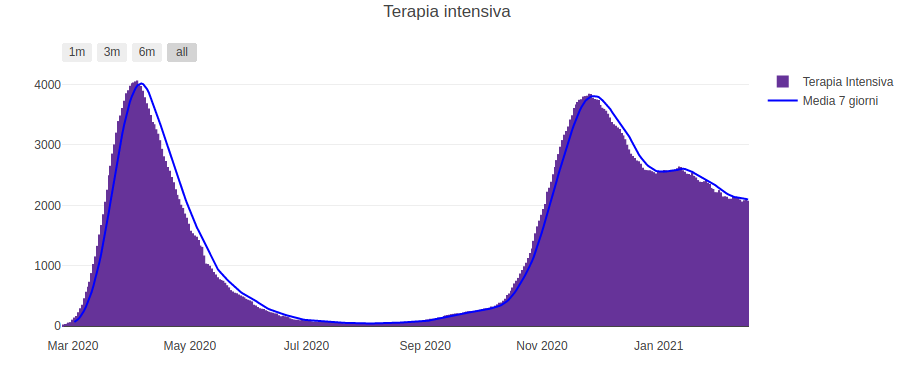
\includegraphics[width=14cm]{terapia_intensiva}
    \caption{Terapia intensiva}
    \label{fig:terapia_intensiva}
\end{figure}

\subsection{Casi normalizzati}
Il grafico nella figura \ref{fig:casi_normalizzati} mostra il numero di casi normalizzati, ossia resi indipendenti dai tamponi effettuati ogni giorno.
In arancione è indicata anche la linea della media mobile a 7 giorni.
\begin{figure}[htp]
    \centering
    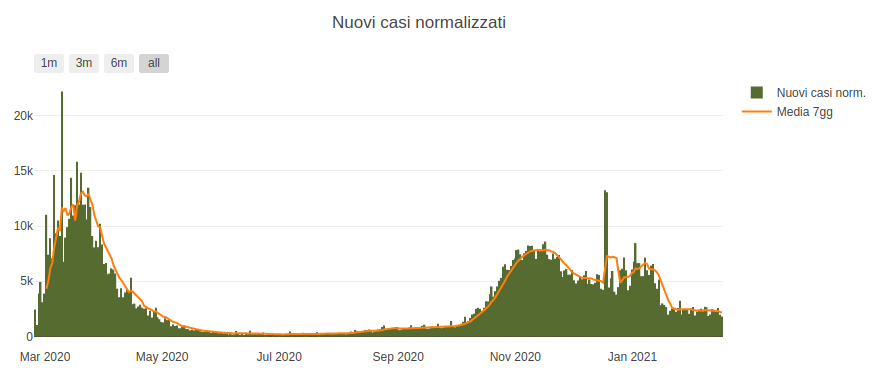
\includegraphics[width=14cm]{casi_norm}
    \caption{Casi normalizzati}
    \label{fig:casi_normalizzati}
\end{figure}

\subsection{Terapia intensiva e ospedalizzati}
Nel grafico della figura \ref{fig:ti_ospdedalizzati} è possibile osservare l'andamento delle persone ospedalizzate, cioè la somma dei ricoverati con sintomi e di quelli in terapia intensiva.
\begin{figure}[htp]
    \centering
    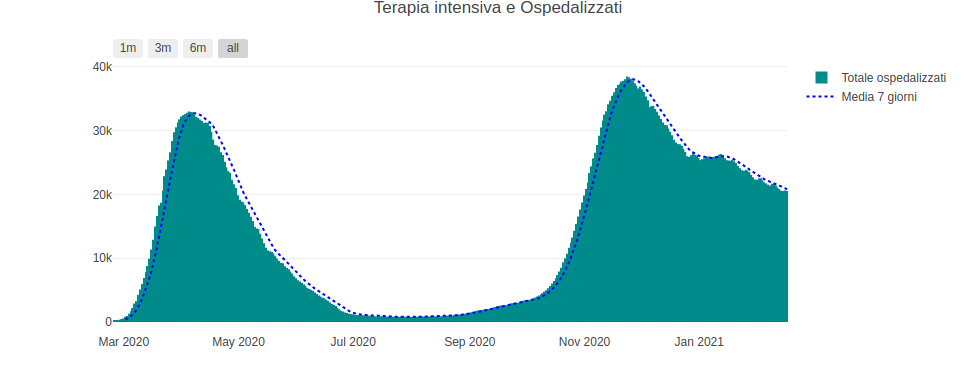
\includegraphics[width=14cm]{ospedalizzati}
    \caption{Terapia intensiva e ospedalizzati}
    \label{fig:ti_ospdedalizzati}
\end{figure}

\subsection{Decessi e contagi giornalieri}
Nella figura \ref{fig:decessi_contagi_medie} è rappresentato l'andamento dei decessi (linea blu punteggiata) e dei contagi giornalieri (linea arancione punteggiata).
Le linee blu e arancione sono rispettivamente la media mobile a 7 giorni per decessi e contagi giornalieri.
\begin{figure}[htp]
    \centering
    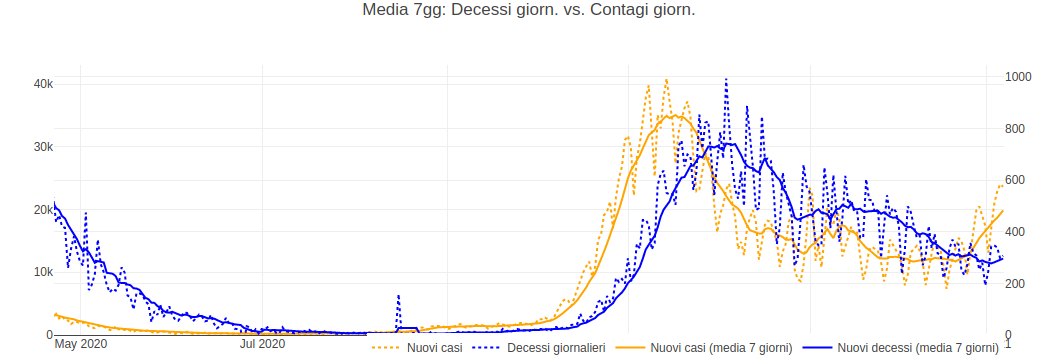
\includegraphics[width=14cm]{img/decessi_vs_contagi.png}
    \caption{Andamento di decessi e contagi}
    \label{fig:decessi_contagi_medie}
\end{figure}

\subsection{Percentuale dei casi positivi sui casi testati}
Nella figura \ref{fig:casi_pos_testati_italy} si può osservare l'andamento della percentuale dei casi positivi sui casi testati con tamponi.
\begin{figure}[htp]
    \centering
    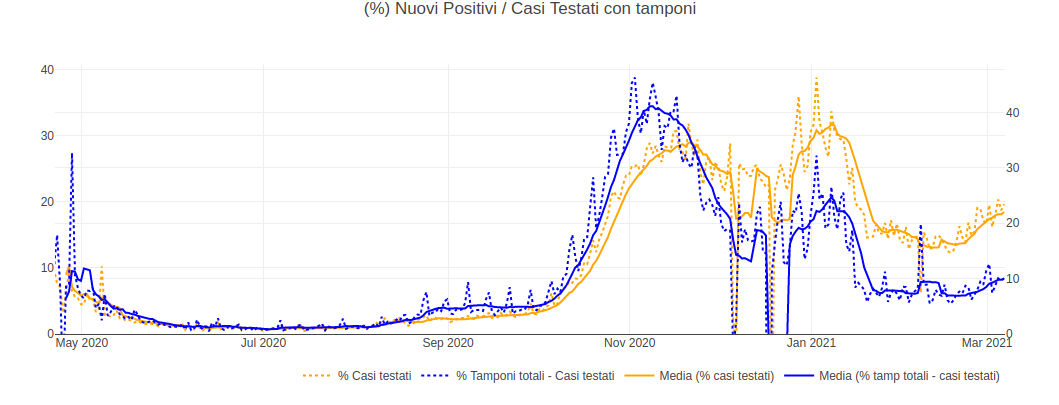
\includegraphics[width=14cm]{img/positivi_testati.png}
    \caption{Percentuale dei nuovi positivi sui casi testati}
    \label{fig:casi_pos_testati_italy}
\end{figure}

\subsection{Nuovi casi e decessi}
Nella figura \ref{fig:casi_decessi} viene mostrato l'andamento dei positivi e dei decessi.
In questo grafico è anche possibile selezionare l'intervallo temporale, agendo sulla barra in basso.
\begin{figure}[htp]
    \centering
    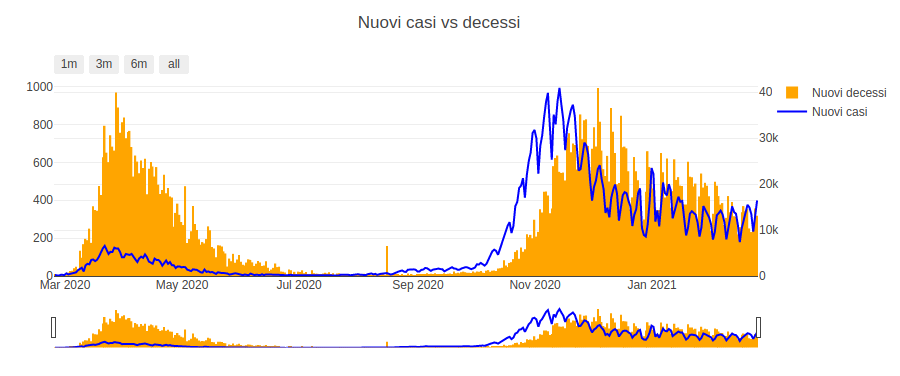
\includegraphics[width=14cm]{casi_decessi}
    \caption{Nuovi casi e nuovi decessi}
    \label{fig:casi_decessi}
\end{figure}

\section{Dashboard Lombardia}
\subsection{Andamento dei contagi}
Nella figura \ref{fig:andamento_lomb} è raffigurato l'andamento dei contagi nella regione Lombardia.
In giallo la linea della media mobile a 7 giorni.
\begin{figure}[htp]
    \centering
    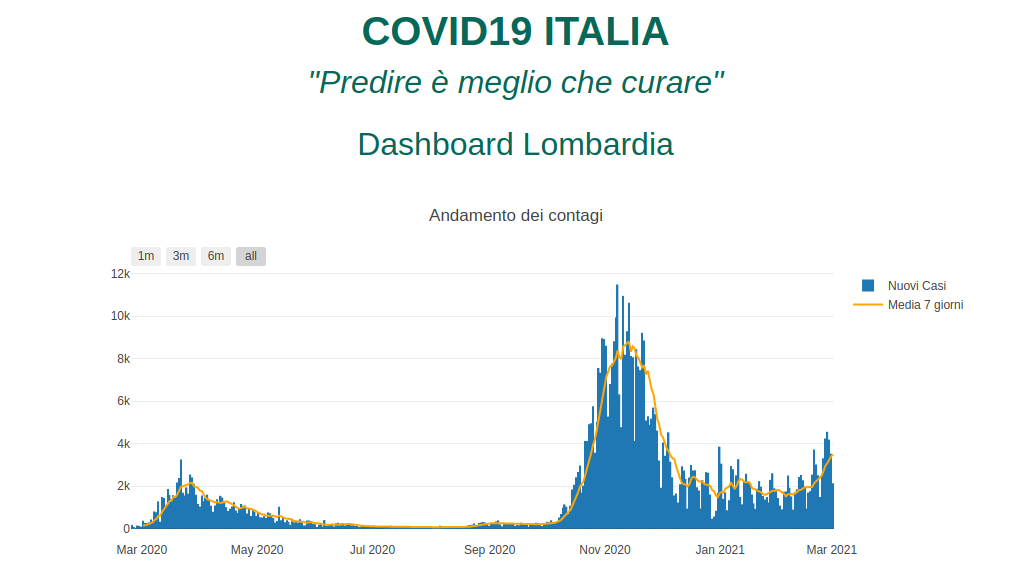
\includegraphics[width=12cm]{img/lomb/andamento_lomb.png}
    \caption{Andamento dei contagi in Lombardia}
    \label{fig:andamento_lomb}
\end{figure}

\subsection{Percentuale positivi sui casi testati}
La figura \ref{fig:positivi_testati_lomb} rappresenta la percentuale del rapporto tra i nuovi casi rispetto al totale dei casi e al numero dei casi testati tramite tamponi.
La linea gialla indica l'andamento dei \emph{nuovi casi testati}, mentre quella blu indica il \emph{totale dei casi testati}.
Le linee "punteggiate" indicano le medie mobili a 3 giorni.
\begin{figure}[htp]
    \centering
    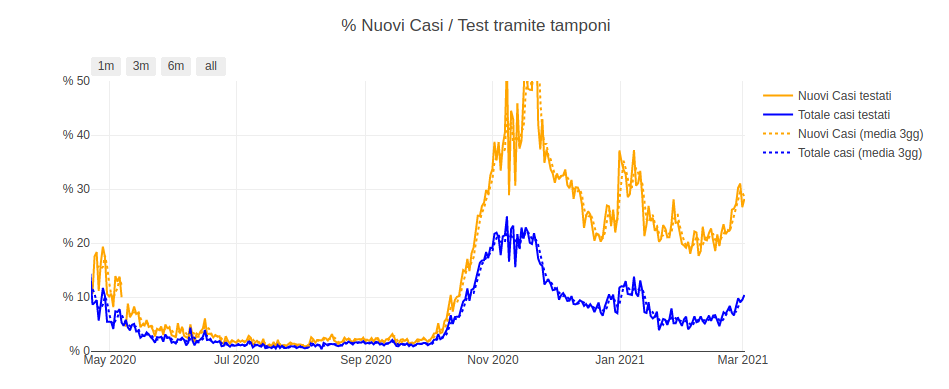
\includegraphics[width=12cm]{img/lomb/casi_tamp_lomb.png}
    \caption{Andamento dei contagi in Lombardia}
    \label{fig:positivi_testati_lomb}
\end{figure}

\subsection{Casi normalizzati}
Nella figura \ref{fig:casi_norm_lomb} è possibile osservare l'andamento dei casi normalizzati nella regione Lombardia.
\begin{figure}[htp]
    \centering
    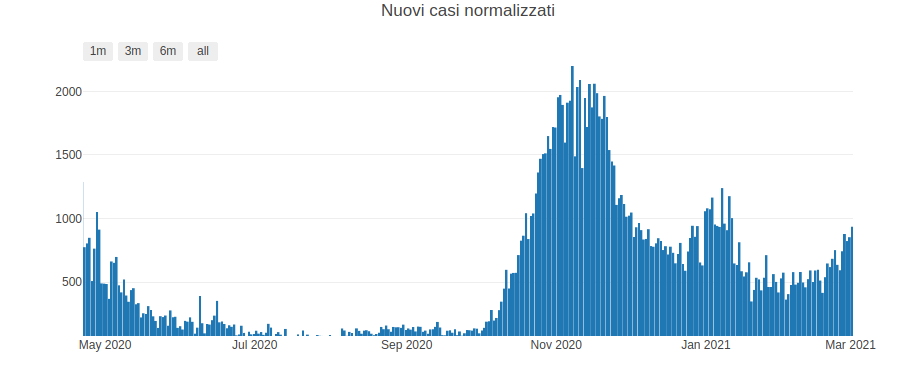
\includegraphics[width=14cm]{img/lomb/casi_norm_lomb.png}
    \caption{Andamento dei casi normalizzati}
    \label{fig:casi_norm_lomb}
\end{figure}

\subsection{Ospedalizzazioni}
Nella figura \ref{fig:ospedalizzati_lomb} si può osservare l'andamento delle ospedalizzazioni nella regione Lombardia.
In arancione la linea della media mobile a 7 giorni.
\begin{figure}[htp]
    \centering
    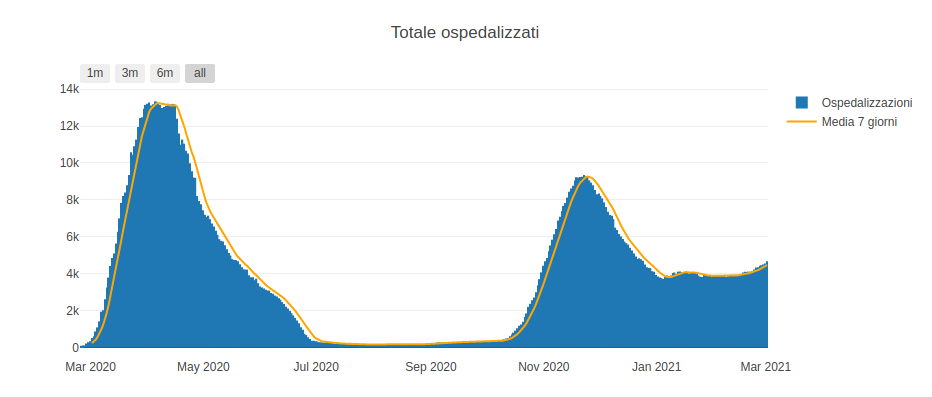
\includegraphics[width=14cm]{img/lomb/ospedalizzati_lomb.png}
    \caption{Andamento delle ospedalizzazioni in Lombardia}
    \label{fig:ospedalizzati_lomb}
\end{figure}

\subsection{Decessi giornalieri}
La figura \ref{fig:decessi_lomb} mostra l'andamento dei decessi nella regione Lombardia.
La linea blu indica la media mobile a 7 giorni.
\begin{figure}[htp]
    \centering
    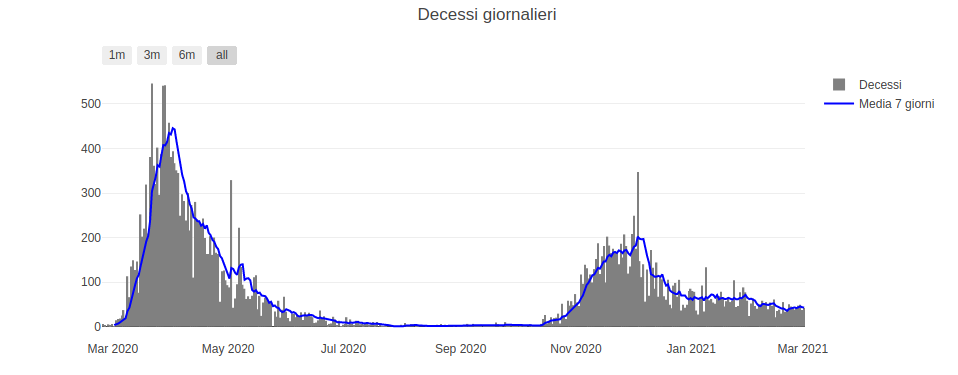
\includegraphics[width=14cm]{img/lomb/decessi_lomb.png}
    \caption{Andamento dei deceduti}
    \label{fig:decessi_lomb}
\end{figure}

\subsection{Terapia intensiva}
La figura \ref{fig:ti_lomb} mostra l'andamento dei pazienti ricoverati negli ospedali lombardi in terapia intensiva dall'inizio della pandemia.
\begin{figure}[htp]
    \centering
    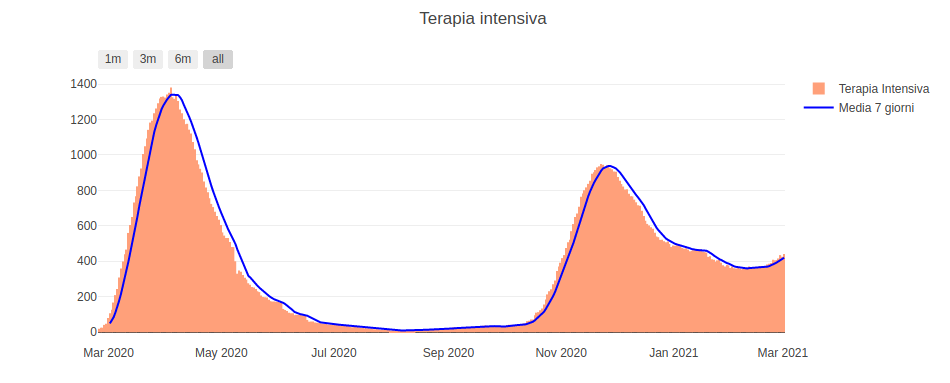
\includegraphics[width=12cm]{img/lomb/ti_lomb.png}
    \caption{Andamento della terapia intensiva}
    \label{fig:ti_lomb}
\end{figure}

\section{Dashboard Regioni}
Nella dashboard regioni, selezionando dal menù a tendina il nome della regione d'interesse (nella figura \ref{fig:tendina}), è possibile visualizzarne i dati.
I grafici contenuti all’interno della dashboard regioni sono analoghi ai precedenti, e riguardano:
\begin{itemize}
\item Andamento dei contagi
\item Percentuale nuovi casi sui tamponi effettuati
\item Totale ospedalizzati
\item Decessi giornalieri
\item Terapia intensiva
\end{itemize}
\begin{figure}[htp]
    \centering
    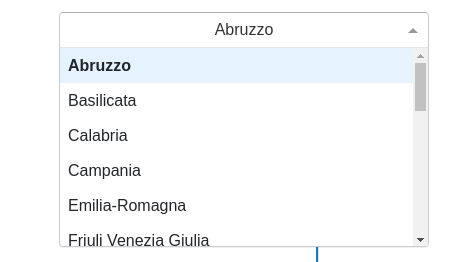
\includegraphics[width=10cm]{img/tendina_regioni.png}
    \caption{Selezione della regione}
    \label{fig:tendina}
\end{figure}

\begin{figure}[htp]
    \centering
    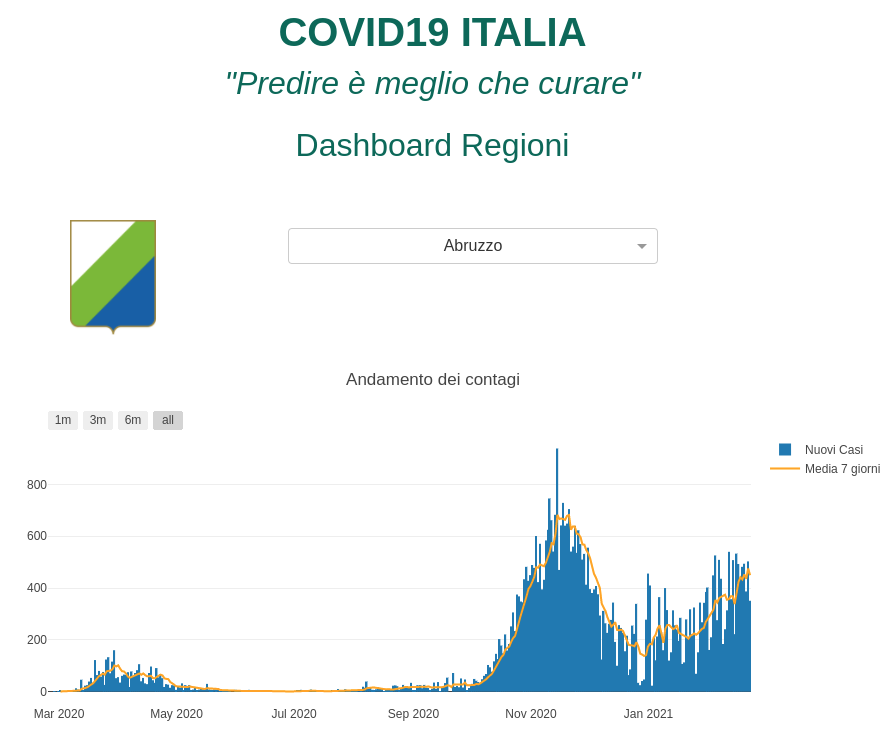
\includegraphics[width=12cm]{dash_regioni}
    \caption{Visualizzazione della regione Abruzzo}
    \label{fig:dash_regioni}
\end{figure}
\mcchap{Il portale Covid19-Italy}{cap:portale}

\noindent Con il patrocinio dell’Università degli studi dell’Insubria è stato ideato il portale Covid 19-Italy.it\footnote{https://covid19-italy.it}, un sito che permette di visualizzare i dati aggregati e ufficiali sull’andamento della pandemia regione per regione e a livello nazionale, attraverso grafici e confronti.
\noindent Sulla pagina principale del sito sono presenti 4 card, che permettono di accedere alle seguenti pagine:
\begin{itemize}
\item \emph{Italy R0(t) Indices} permette di accedere alla pagina sulla stima degli indici di riproduzione R0(t) usando il metodo Wallinga and Teunis ,a livello nazionale,  regioni e per provincia.
\item \emph{Italy dashboard} visualizza il monitoraggio del Covid-19 in Italia, attraverso 9 diversi grafici, sempre aggiornati con la pubblicazione di nuovi dati;
\item \emph{Lombardy dashboard} visualizza l’andamento nella pandemia in dettaglio nella regione Lombardia;
\item \emph{Region dashboard} mostra l’andamento della pandemia in una regione italiana a scelta.
\end{itemize}
\begin{figure}[htp]
    \centering
    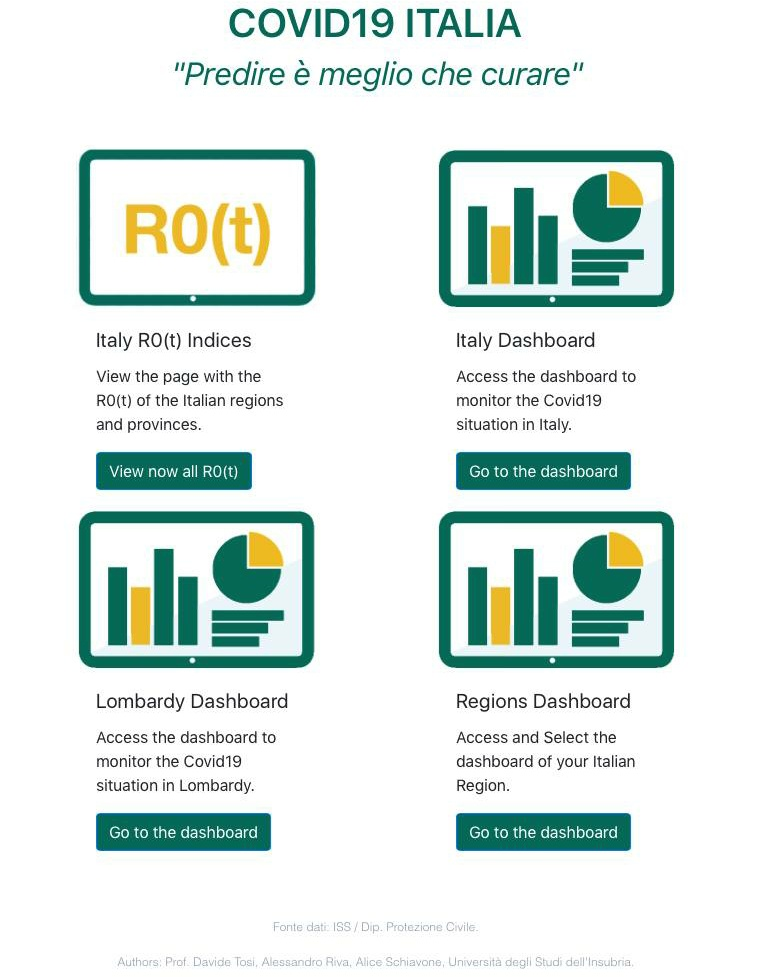
\includegraphics[width=14cm]{covid_19_italy_compact}
    \caption{Pagina principale del sito}
    \label{fig:home_page}
\end{figure}


\mcchap{Conclusioni}{cap:conclusion}

\noindent Lo scopo dell’elaborato di tesi era quello di illustrare la struttura dell'applicazione creata per la visualizzazione dei grafici sulla pandemia di Covid-19.\\
Gli obiettivi prefissati sono stati raggiunti con successo attraverso la realizzazione di una dashboard utilizzando il linguaggio open source Python 3.\\
A causa dell’emergenza sanitaria tutt’ora in corso, il tirocinio si è svolto a distanza, in modalità \emph{smart working}.\\
Questa situazione non ne ha condizionato in modo negativo lo svolgimento, in quanto sono sempre rimasto in contatto con il mio tutor.\\
Lavorare su questo progetto mi ha permesso di acquisire nuove conoscenze e mettere in pratica le mie abilità.
\noindent La pandemia di Covid19 ha stravolto le nostre vite, ha cambiato il modo di lavorare e comunicare.

\begin{appendices}
\mcchap{Manuale utente}{cap:manuale}

\section{Esecuzione in locale}

\subsection{Requisiti software}
Il progetto è stato realizzato utilizzando \emph{ambiente di sviluppo integrato} (IDE) Pycharm Community.
Per l'esecuzione della dashboard sono richieste le seguenti dipendenze.
\begin{itemize}
 \item Git
 \item Python 3.8.5
 \item Pandas
 \item Plotly 
 \item Dash 
 \item Dash Bootstrap Components
 \end{itemize}
 
 \subsection{Clonazione del repository}
 E' possibile scaricare il progetto direttamente dal mio repository Github, con il comando \texttt{git clone https://github.com/alex27riva/Covid-dashboard}
 
 \subsection{Installazione dipendenze}
 Per installare le librerie richieste è sufficiente lanciare i seguenti comandi dal termianle integrato in Pycharm.
 
 \begin{itemize}
     \item \texttt{\$ pip install pandas}
     \item \texttt{\$ pip install plotly==4.12.0}
     \item \texttt{\$ pip install dash==1.17.0}
     \item \texttt{\$ pip install dash-bootstrap-components}
 \end{itemize}
 
 \begin{figure}[htp]
    \centering
    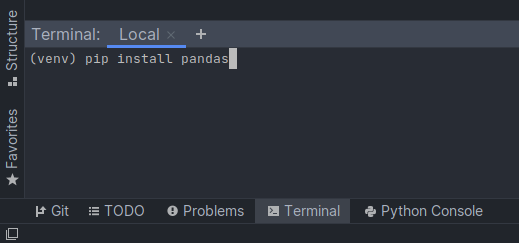
\includegraphics[width=10cm]{pycharm_terminal}
    \caption{Terminale integrato in Pycharm}
    \label{fig:pycharm_termianl}
\end{figure}

Ad installazione completata, sarà possibile avviare il progetto.

\subsection{Avvio del programma}

Per avviare il programma basta premere sul pulsante con la freccina verde.
Verrà avviato un server locale, il cui suo URL verrà mostrato nella console di debug a cui si potrà visualizzare la pagina della dashboard.

 \begin{figure}[htp]
    \centering
    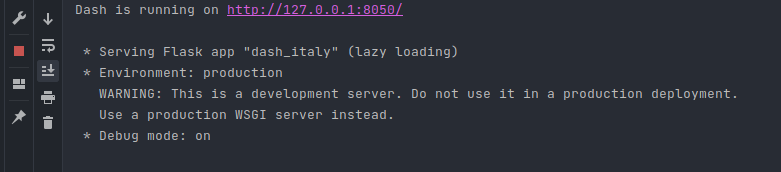
\includegraphics[width=9cm]{running_program}
    \caption{Programma Python in esecuzione}
    \label{fig:running_program}
\end{figure}

\section{Configurazione della VPS}
E' necessario disporrre di un server privato virtuale (VPS) con sistema operativo Ubuntu Server.

\subsection{Creazione account utente}
Per questioni di sicurezza è meglio non utilizzare l'account privilegiato \emph{root}.
\begin{enumerate}
\item Collegarsi alla VPS tramite SSH \texttt{ssh root@<ip-della-VPS>}
\item Crea l'account per l'utente admin \texttt{useradd -m admin}
\item Imposta una password per l'utente admin \texttt{passwd admin}
\item Chiudi la connessione con il comando \texttt{exit}
\end{enumerate}

\subsection{Installazione di Docker}

\begin{enumerate}
\item Collegati alla VPS con l'account admin \texttt{ssh admin@<ip-della-VPS>}
\item Scarica lo script per l'installazione di Docker \texttt{curl -fsSL https://get.docker.com -o get-docker.sh}
\item Esegui lo script con \texttt{sudo sh get-docker.sh}
\item Esegui questo comando per interagire con Docker senza previlegi di root \texttt{sudo usermod -aG docker admin}
\end{enumerate}

\subsection{Installazione e avvio dei container}
I container con le tre dashboard sono presenti nei repository di Docker, è sufficiente eseguire i seguenti comandi per la loro installazione e avvio.
\begin{itemize}
\item \texttt{docker run -d -p 8050:8050 --name=dashboard\_italy alex27riva/dash\_italy}
\item \texttt{docker run -d -p 8051:8050 --name=dashboad\_lomb alex27riva/dashboard\_lombardia}
\item \texttt{docker run -d -p 8052:8050 --name=dashboard\_regioni alex27riva/dashboard\_regioni}
\end{itemize}

\subsection{Portainer}
Per una gestione più semplice dei container Docker è possibile installare Portainer, un interfaccia web che facilita l'avvio, aggiornamento, rimozione dei container.
Per installare Portainer sono necessari questi due comandi:
\begin{enumerate}
    \item \texttt{docker volume create portainer\_data}
    \item \texttt{docker run -d -p 8000:8000 -p 9000:9000 --name=portainer --restart=always\\ -v /var/run/docker.sock:/var/run/docker.sock -v portainer\_data:/data\\ portainer/portainer-ce}
\end{enumerate}

Ora si può collegarsi all'interfaccia web all'indirizzo \emph{http://\textless ip-vps\textgreater:9000}

\subsection{Ngnix}
Ngnix è un web server, che è stato utilizzato come reverse proxy.

\subsubsection*{Installazione di Ngnix}

\begin{enumerate}
    \item \texttt{sudo apt update}
    \item \texttt{sudo apt install nginx}
    \item \texttt{unlink /etc/nginx/sites-enabled/default}
    \item \texttt{sudo nano /etc/nginx/sites-available/reverse-proxy.conf}
\end{enumerate}

\begin{lstlisting}[basicstyle=\ttfamily\small]
server
 {
    listen 80;
    listen 443;
    listen [::]:80;
    ssl on;
    ssl_certificate /etc/letsencrypt/live/dash.covid19-italy.it/fullchain.pem;
    ssl_certificate_key /etc/letsencrypt/live/dash.covid19-italy.it/privkey.pem;

    server_name dash.covid19-italy.it
    
    access_log /var/log/nginx/reverse-access.log;
    error_log /var/log/nginx/reverse-error.log;
    
    location /italy/ {
                proxy_pass http://localhost:8050;

    }

    location /lombardy/ {
            proxy_pass http://localhost:8051;

    }

    location /regions/ {
            proxy_pass http://localhost:8052;

    }
}
\end{lstlisting}

\subsubsection*{Creazione del link simbolico}
\texttt{\$ ln -s /etc/nginx/sites-available/reverse-proxy.conf\\ /etc/nginx/sites-enabled/reverse-proxy.conf}

\subsubsection*{Test della configurazione}
\texttt{nginx -t}

\subsection*{Installazione certificato SSL}
\begin{enumerate}
\item Assicurarsi che snap sia aggiornato \texttt{sudo snap install core; sudo snap refresh core}
\item Installare Certbot \texttt{sudo snap install --classic certbot}
\item Crea link simbolico per l'eseguibile \texttt{sudo ln -s /snap/bin/certbot /usr/bin/certbot}
\item Richiesta del certificato \texttt{sudo certbot --nginx}
\end{enumerate}

\subsection{riavvio di Nginx}
Riavviare il servizio di Nginx con il seguente comando: \\
\texttt{sudo systemctl restart nginx}


\end{appendices}
\chapter*{Colophon}

Questa tesi è stata scritta in \LaTeX utilizzando Overleaf\footnote{https://overleaf.com}, un editor LaTeX collaborativo basato su cloud utilizzato per scrivere, modificare e pubblicare documenti scientifici.\\
  
\appendix
\backmatter{}
\printindex

\medskip
\nocite{*} % stampa tutta la bibliografia
\printbibliography[
heading=bibintoc,
title={Bibliografia}
]
   
\end{document}